\documentclass[11pt, oneside]{article}   	% use "amsart" instead of "article" for AMSLaTeX format
\usepackage{geometry}                		% See geometry.pdf to learn the layout options. There are lots.
\geometry{letterpaper}                   		% ... or a4paper or a5paper or ... 
%\geometry{landscape}                		% Activate for rotated page geometry
%\usepackage[parfill]{parskip}    		% Activate to begin paragraphs with an empty line rather than an indent
\usepackage{graphicx}				% Use pdf, png, jpg, or eps§ with pdflatex; use eps in DVI mode
								% TeX will automatically convert eps --> pdf in pdflatex		
\usepackage{amssymb}
\usepackage{amsmath}
\usepackage{enumitem}
\usepackage{caption}
\usepackage{subcaption}
\usepackage{multirow}
\usepackage{array}
\usepackage{float}
%\usepackage{enumitem}

%SetFont

%SetFonts


\title{Project \#1}
\author{Huiyu Wang\\604--592--364}
\date{}							% Activate to display a given date or no date

\begin{document}
\maketitle

\begin{figure}[H]
	\centering
	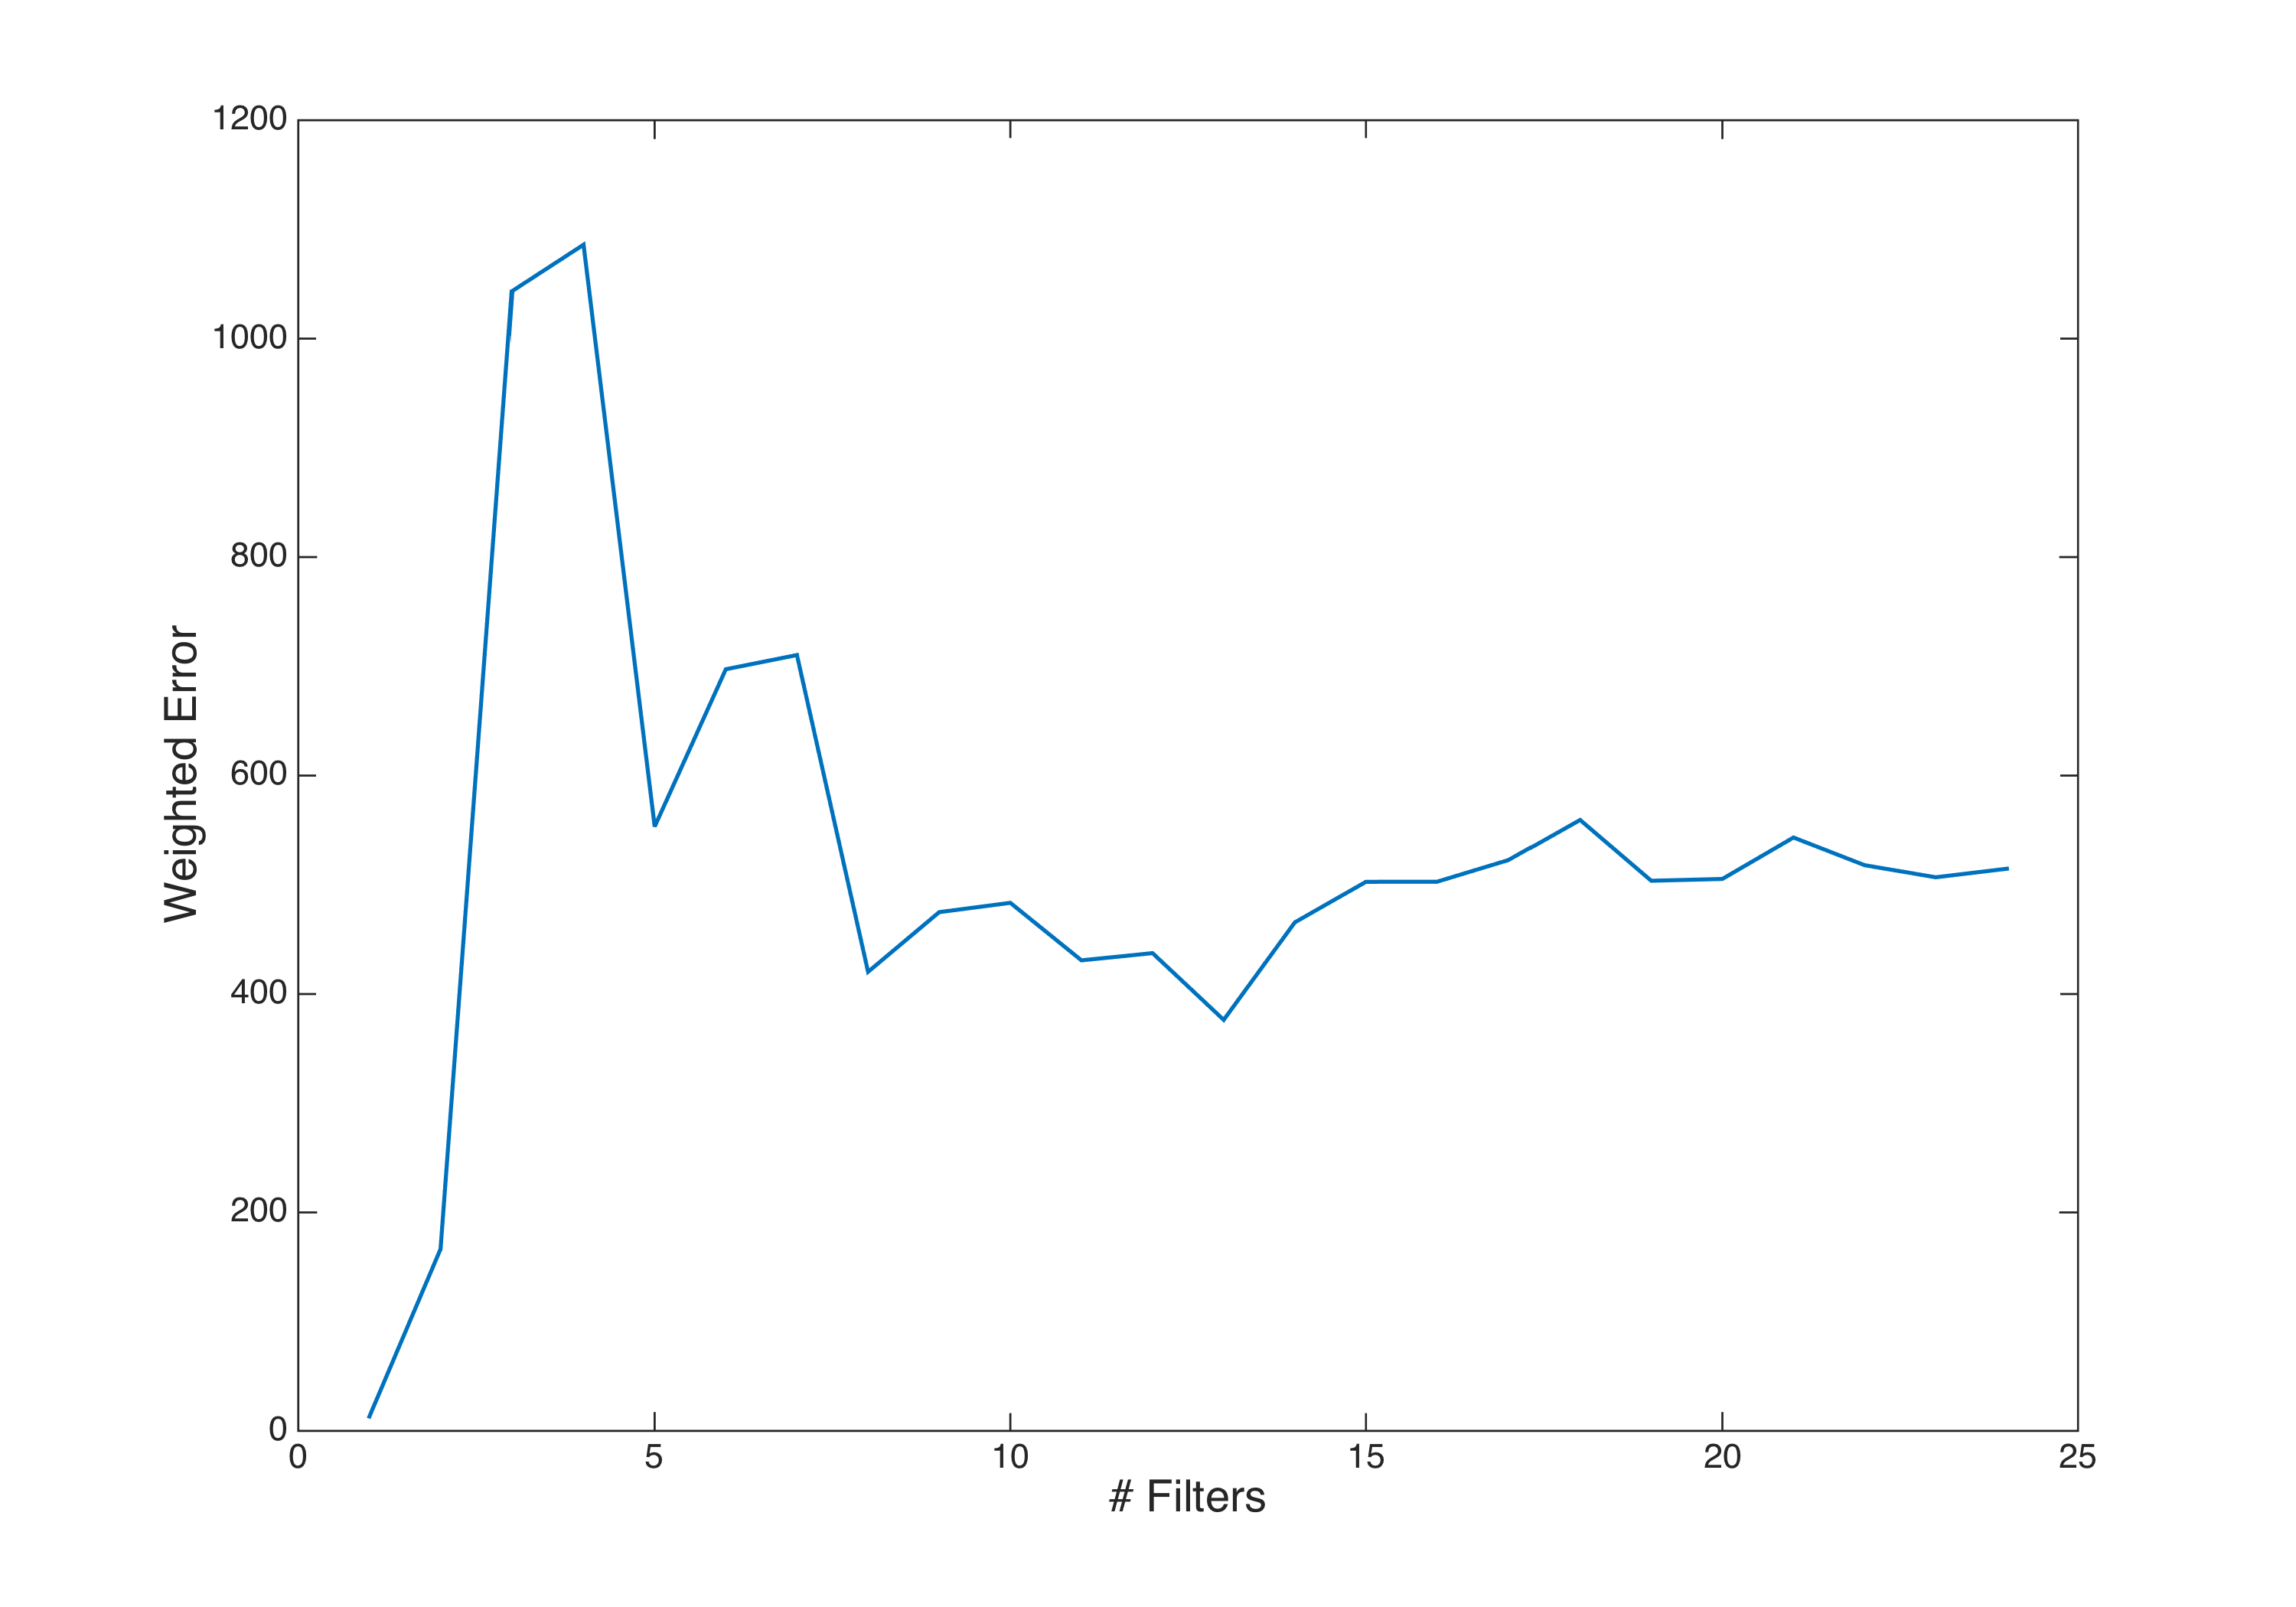
\includegraphics[width=0.8\textwidth]{plot}
	\caption{Per Pixel Error over the number of sweeps or iterations}
	\label {fig:plot}
\end{figure}

Figure \ref{fig:plot} shows the per pixel error of the three methods (Gibbs Sampler L1 norm, Gibbs Sampler L2 norm, PDE Heat Equation).
We can see that the per pixel error of Gibbs Sampler L2 norm decreases faster than that of L1 norm with the same increasing parameter $\beta$, and faster than the PDE Heat Equation (Note that the parameter of heat diffusion equation can affect the decreasing rate of per pixel error and here we use the max stable one which is 0.25). PDE Heat Equation converges to the same error ($\approx$653.9) as Gibbs Sampler L2 norm, as expected, which is less than that of L1 norm. This means the L2 norm potential energy better matches the original image.
\par
Figure \ref{fig:results} shows the restored results of the three methods, including the intermediate results (20 sweeps) and the converged results (100 sweeps).

\begin{figure}[H]
    \centering
    \begin{subfigure}[b]{0.49\textwidth}
        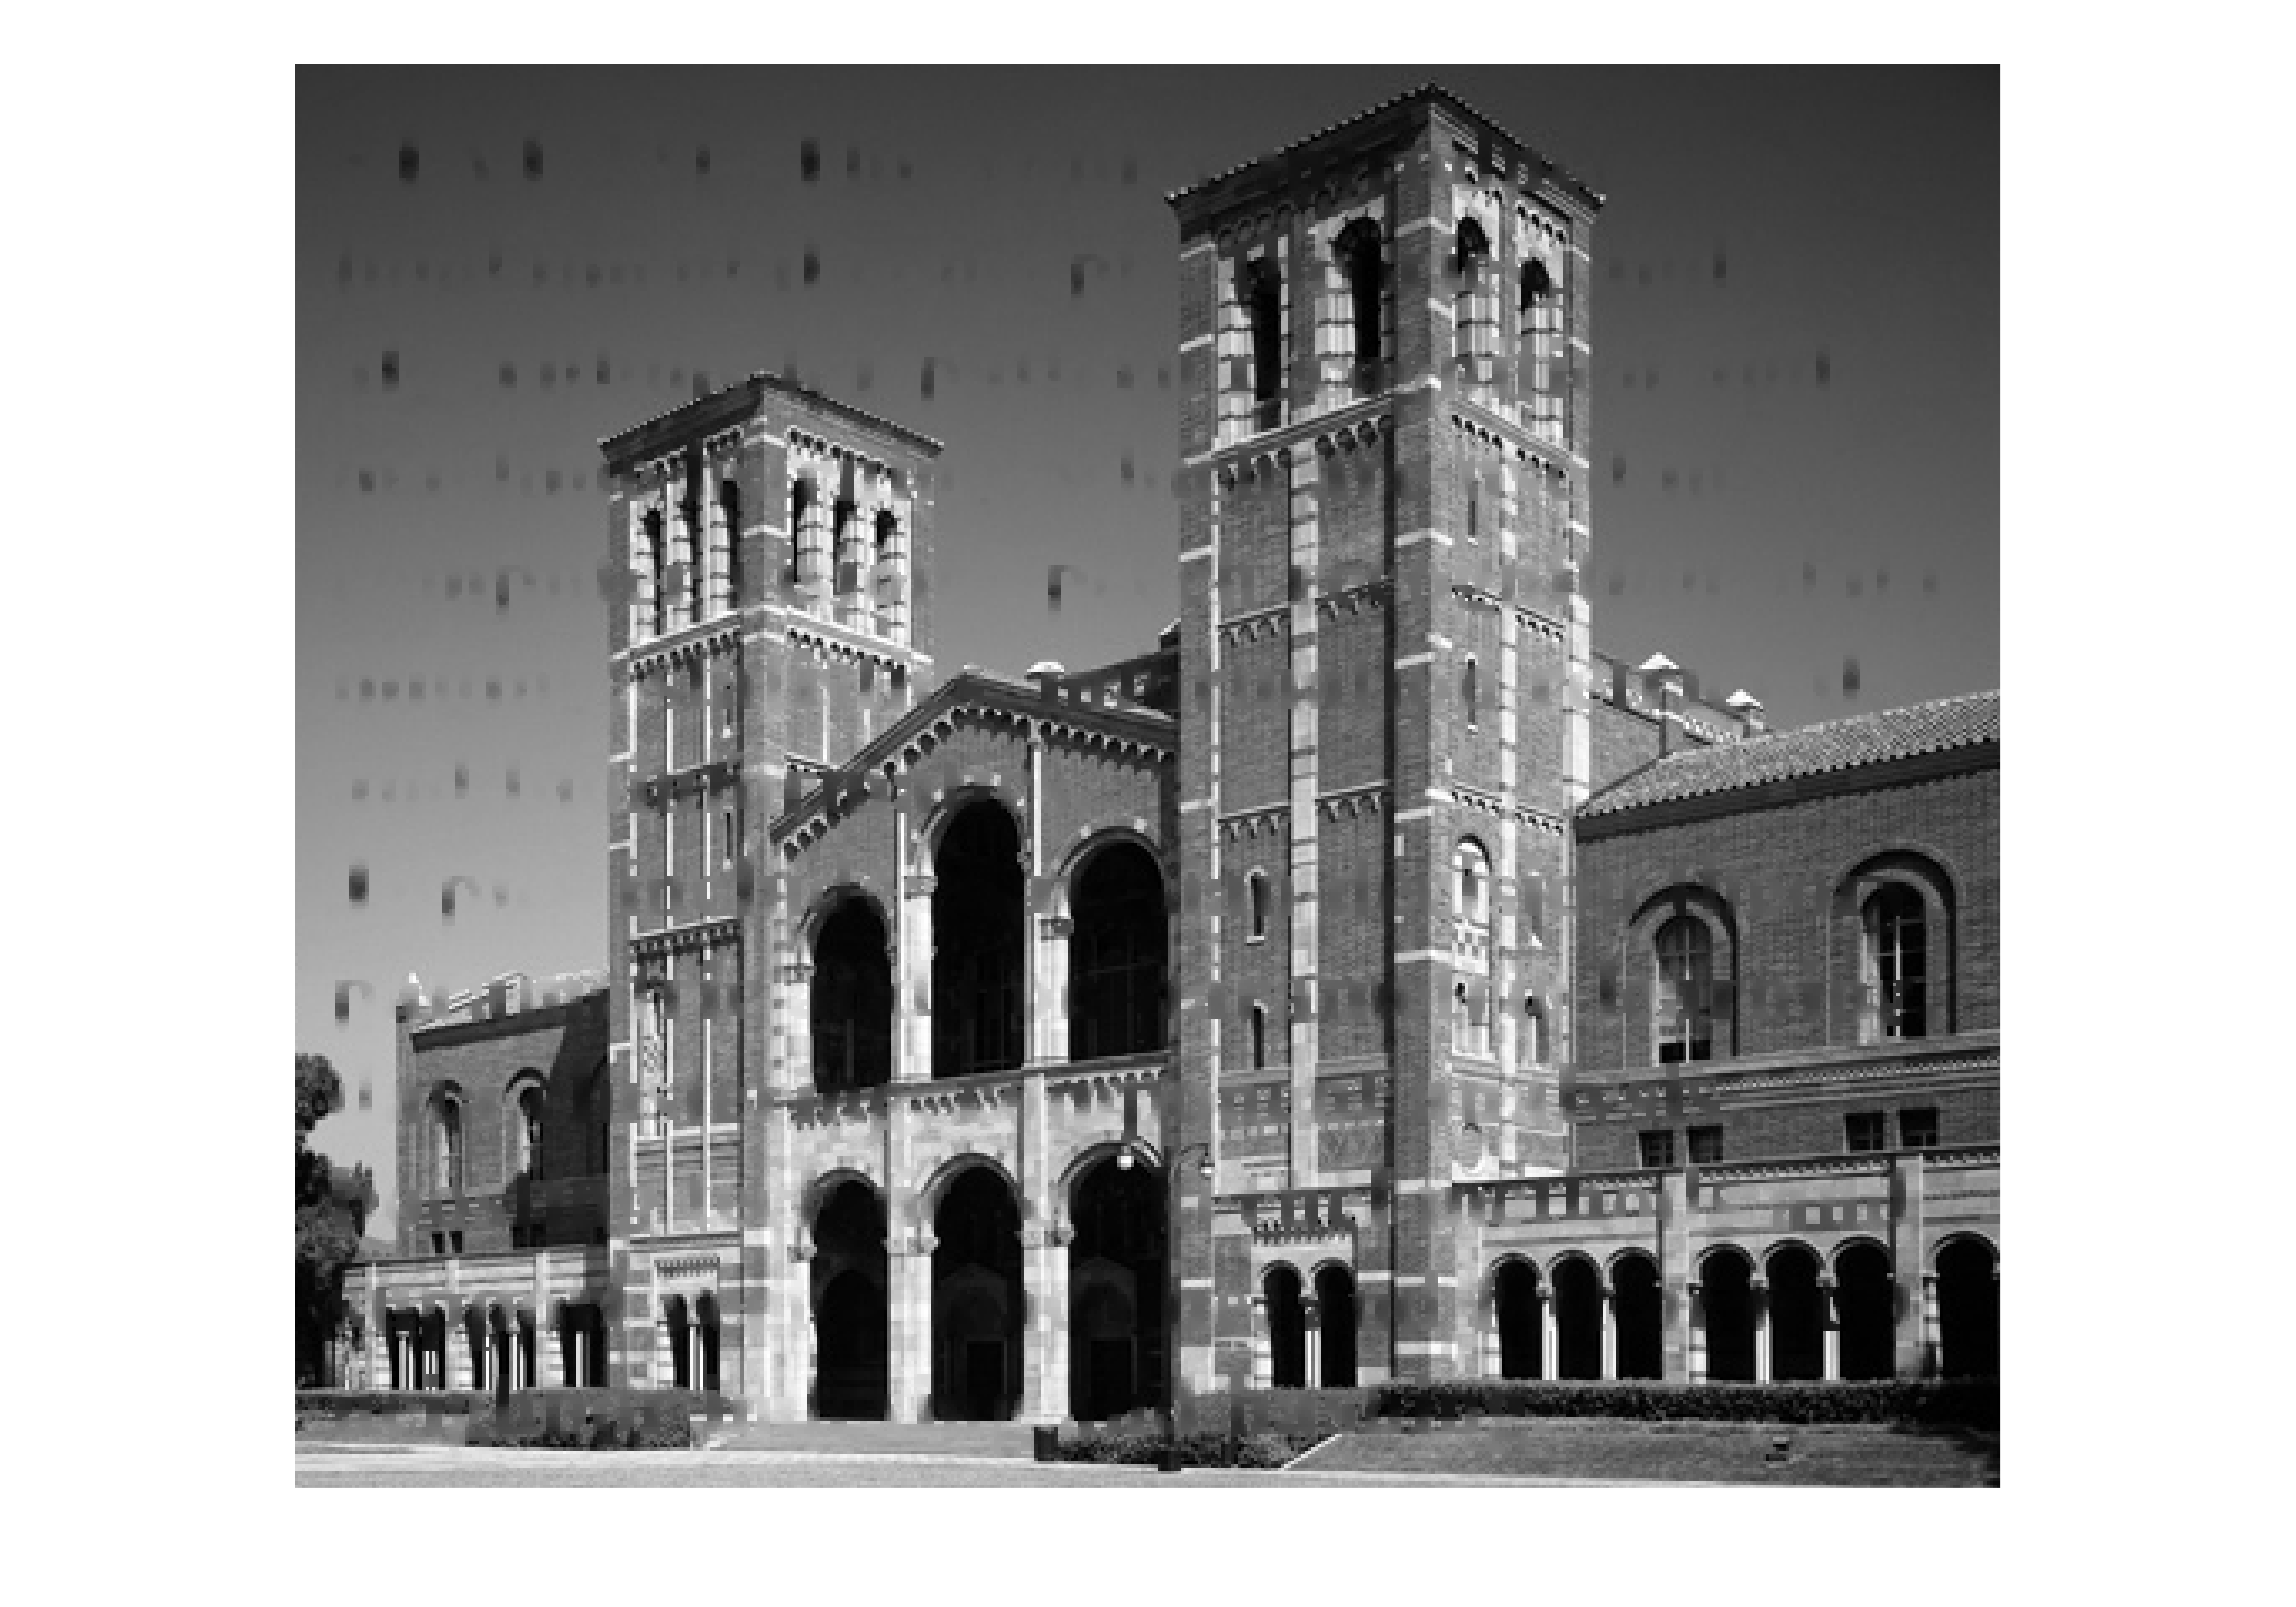
\includegraphics[width=\textwidth]{plot1_20}
        \caption{Gibbs Sampler L1 norm 20 sweeps}
        \label{fig:plot1_20}
    \end{subfigure}
    \begin{subfigure}[b]{0.49\textwidth}
        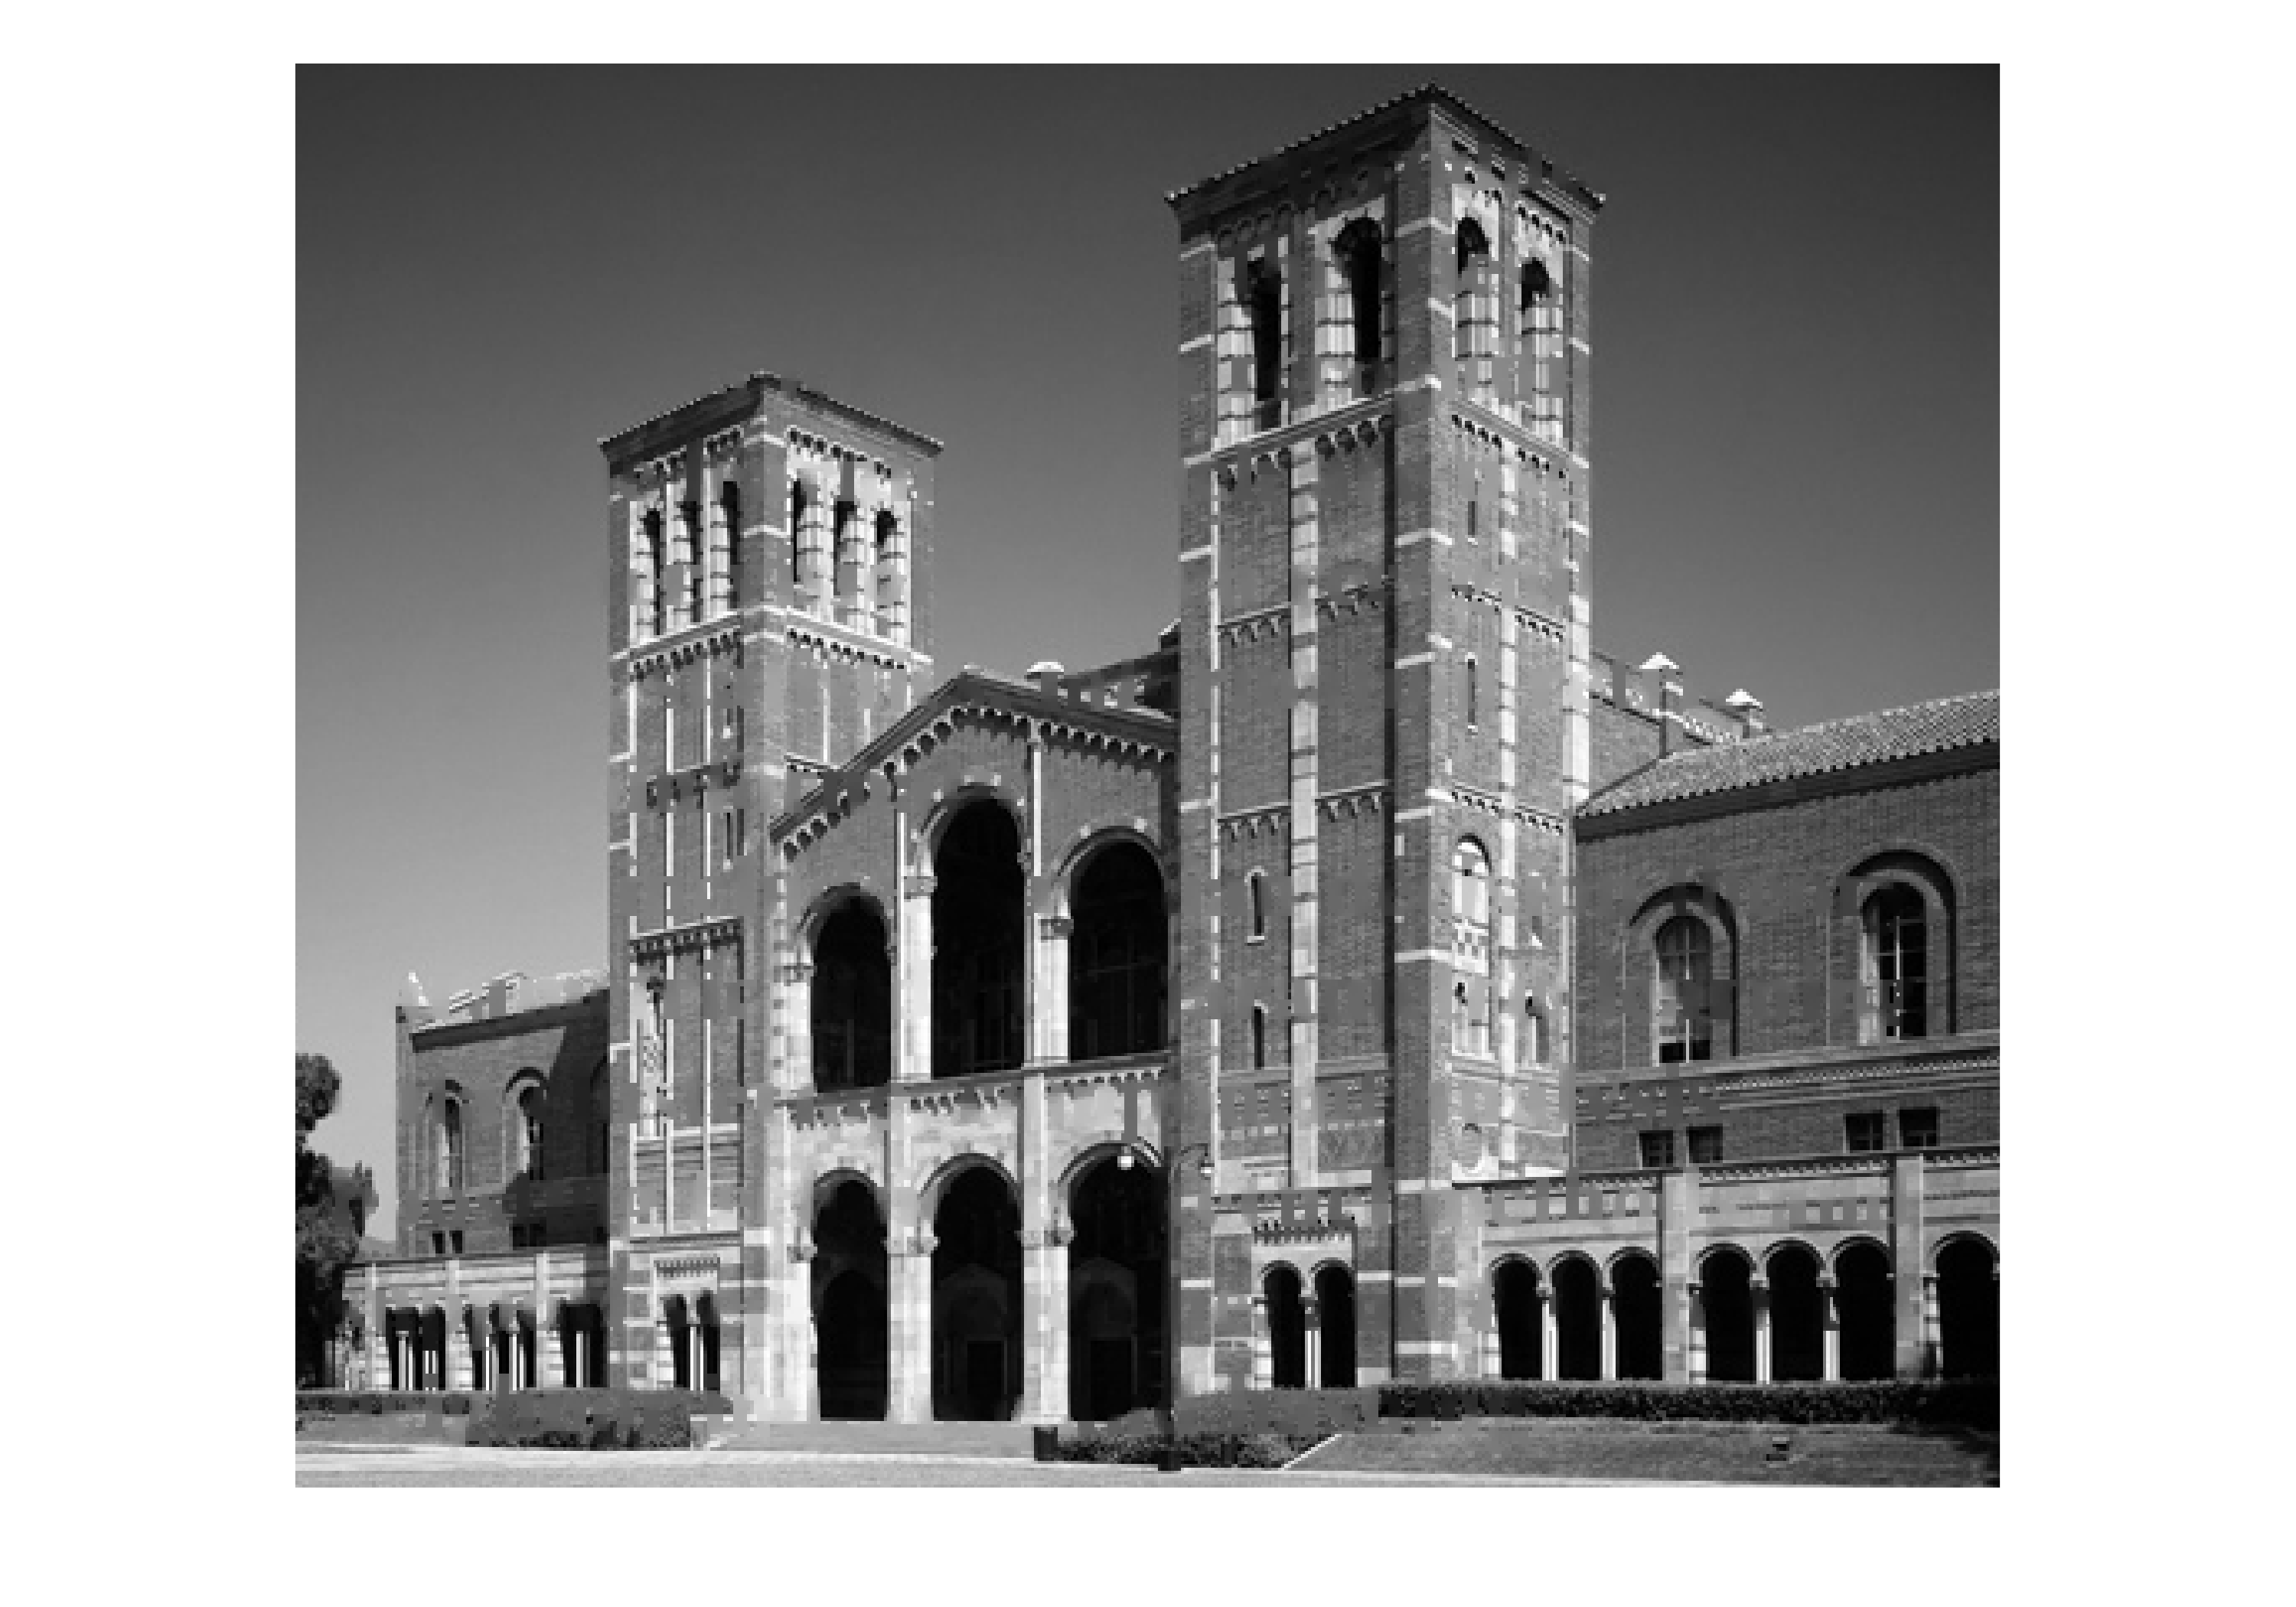
\includegraphics[width=\textwidth]{plot1_100}
        \caption{Gibbs Sampler L1 norm 100 sweeps}
        \label{fig:plot1_100}
    \end{subfigure}
    
    \begin{subfigure}[b]{0.49\textwidth}
        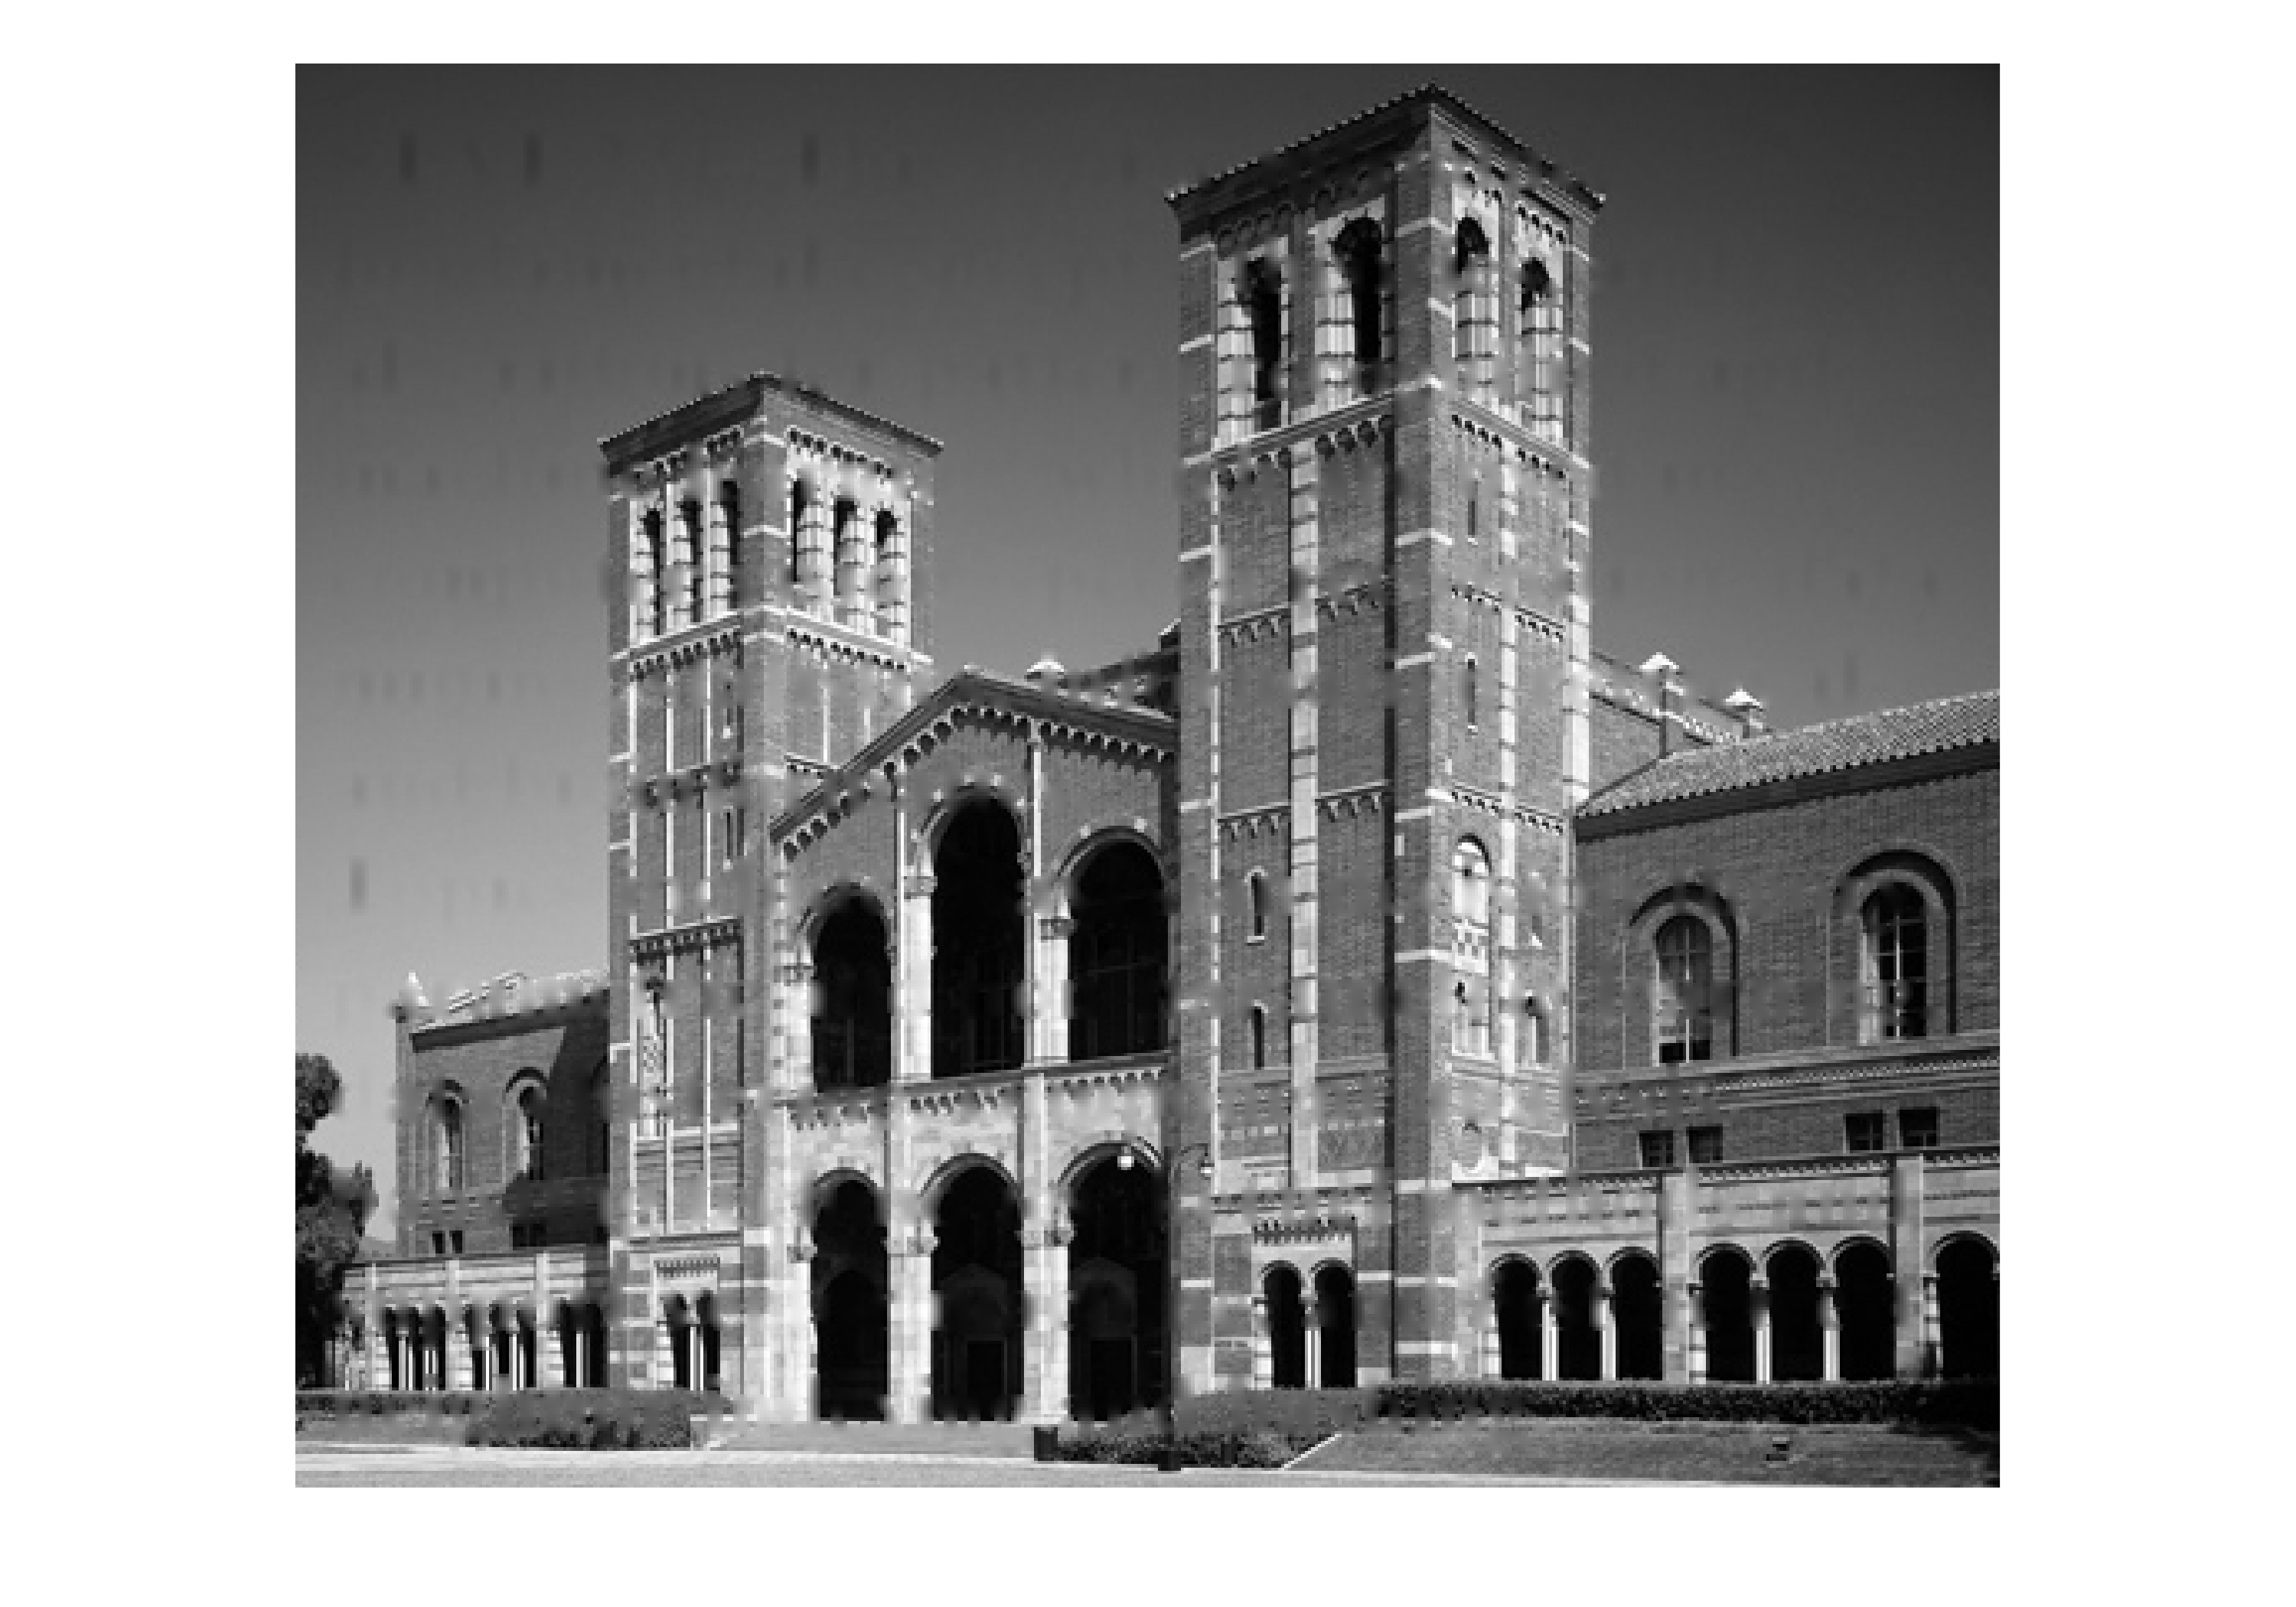
\includegraphics[width=\textwidth]{plot2_20}
        \caption{Gibbs Sampler L2 norm 20 sweeps}
        \label{fig:plot2_20}
    \end{subfigure}
    \begin{subfigure}[b]{0.49\textwidth}
        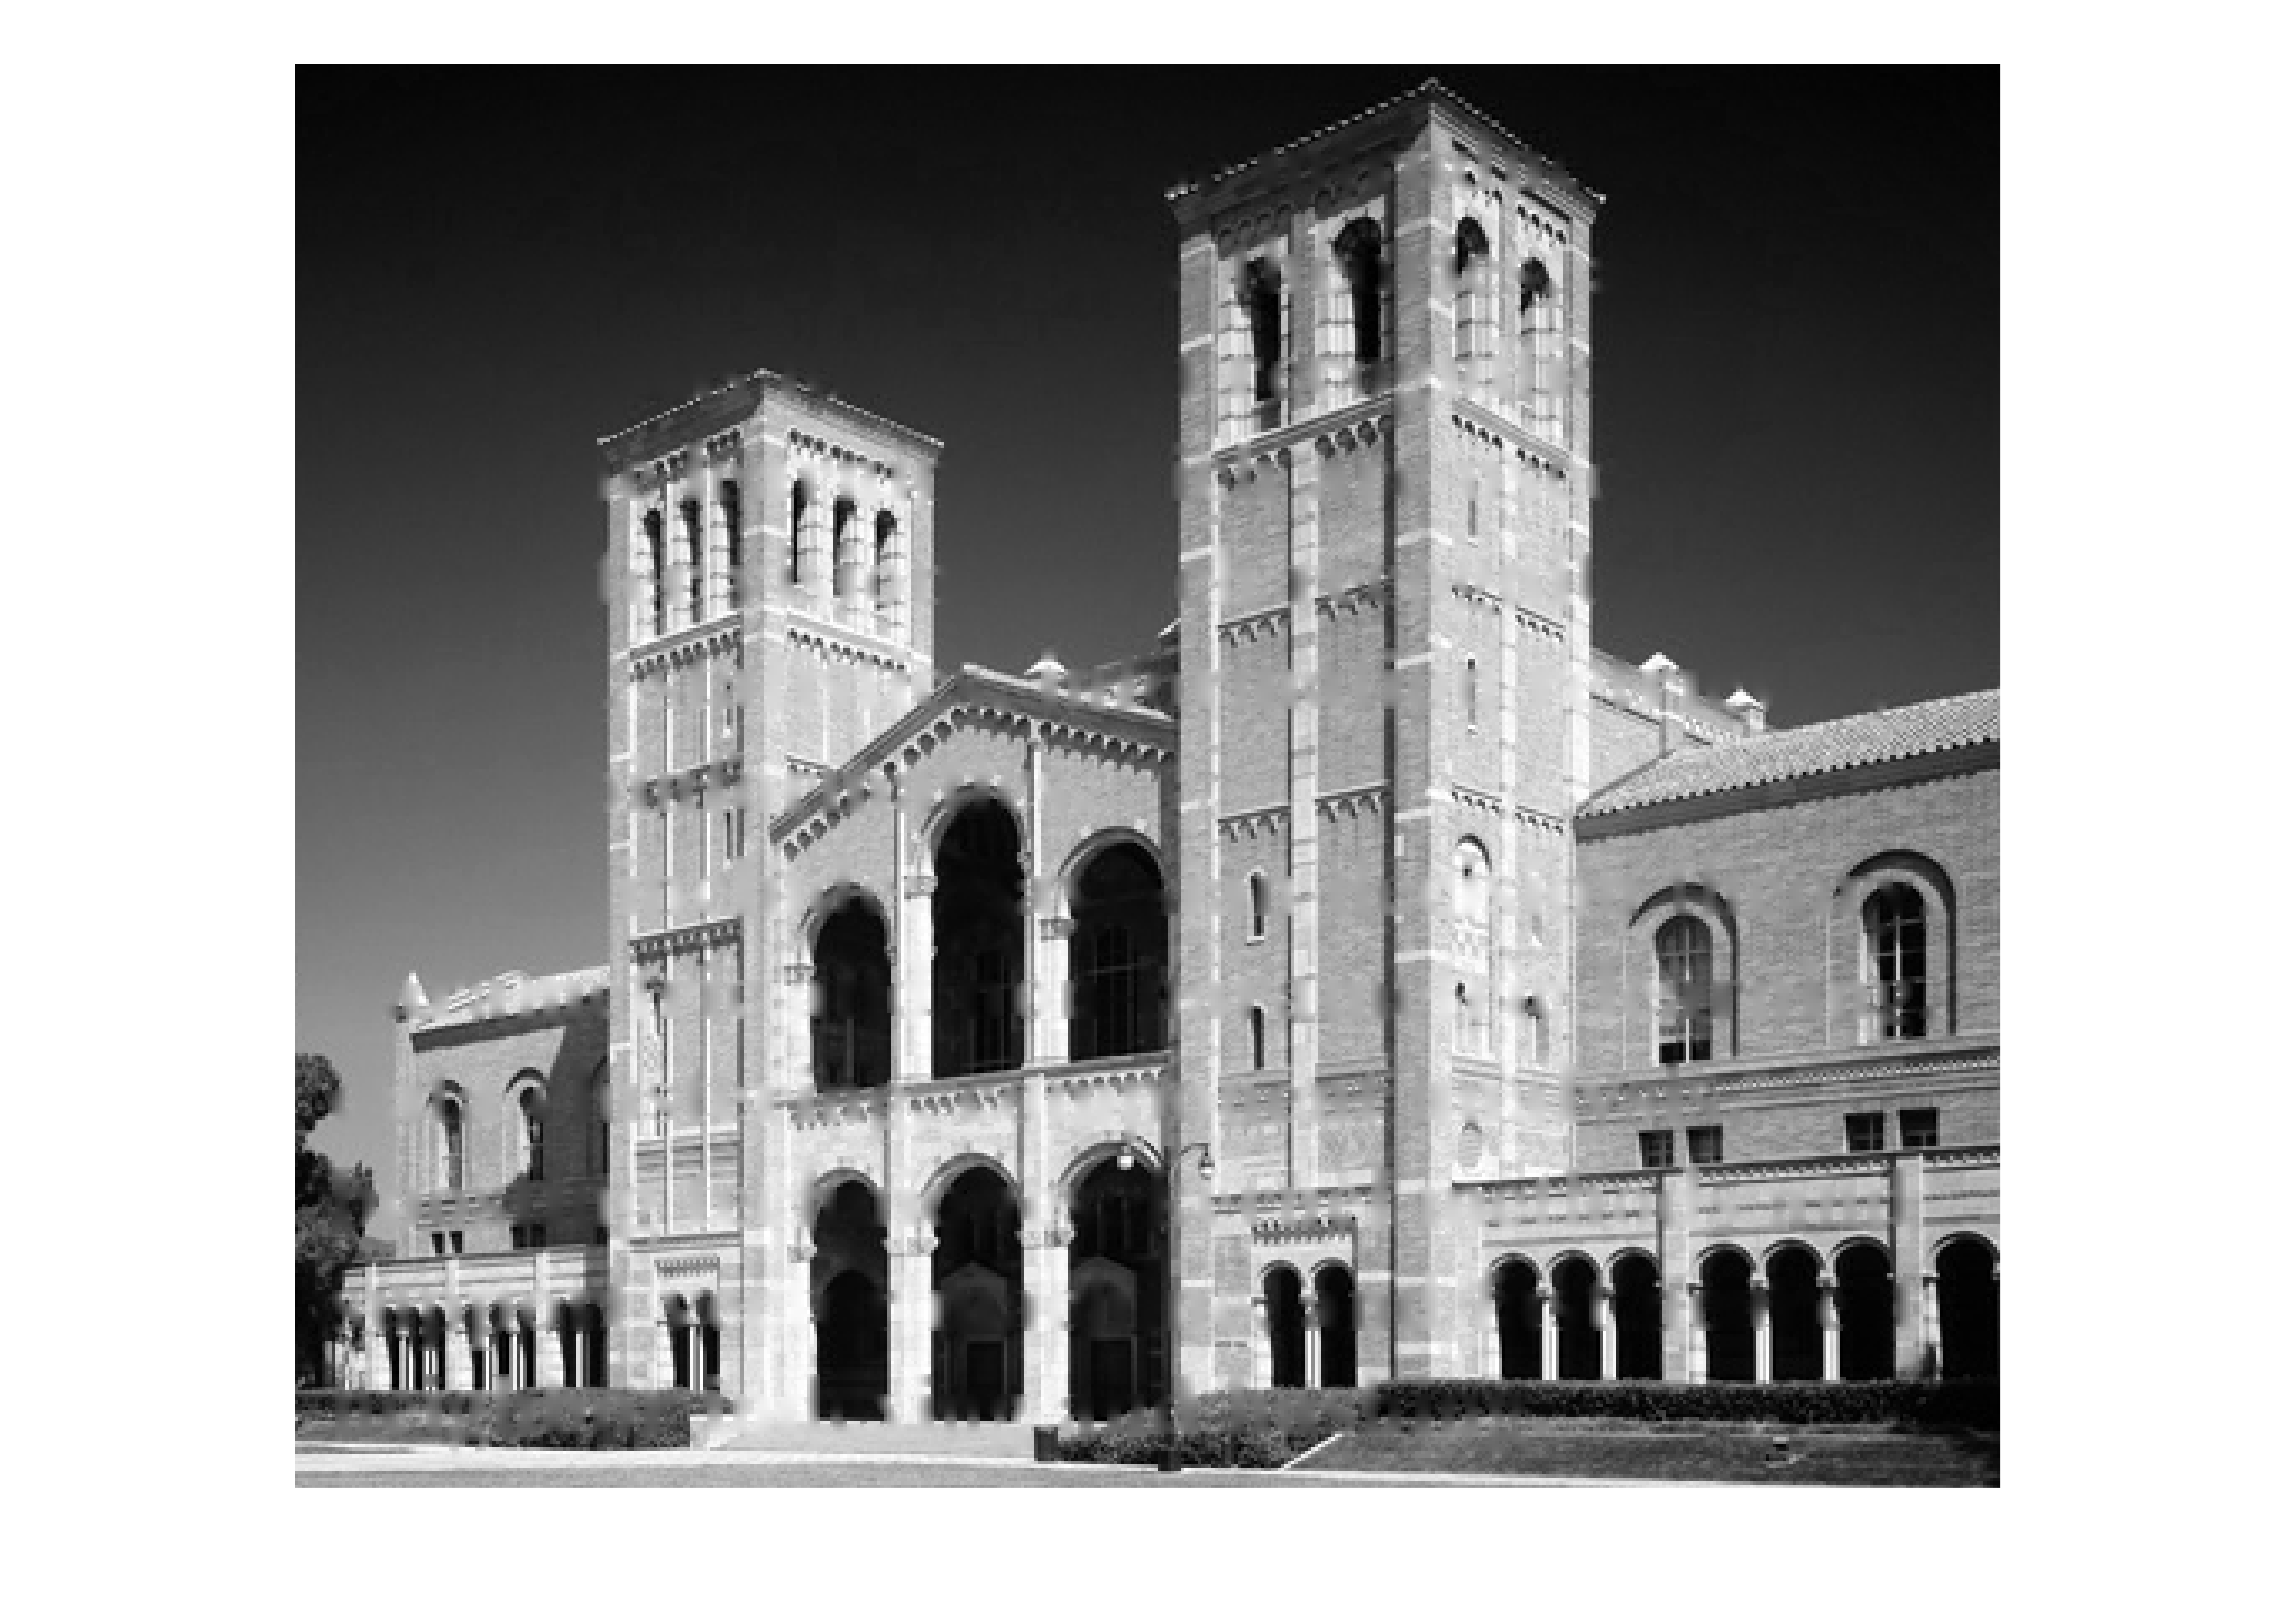
\includegraphics[width=\textwidth]{plot2_100}
        \caption{Gibbs Sampler L2 norm 100 sweeps}
        \label{fig:plot2_100}
    \end{subfigure}
    
    \begin{subfigure}[b]{0.49\textwidth}
        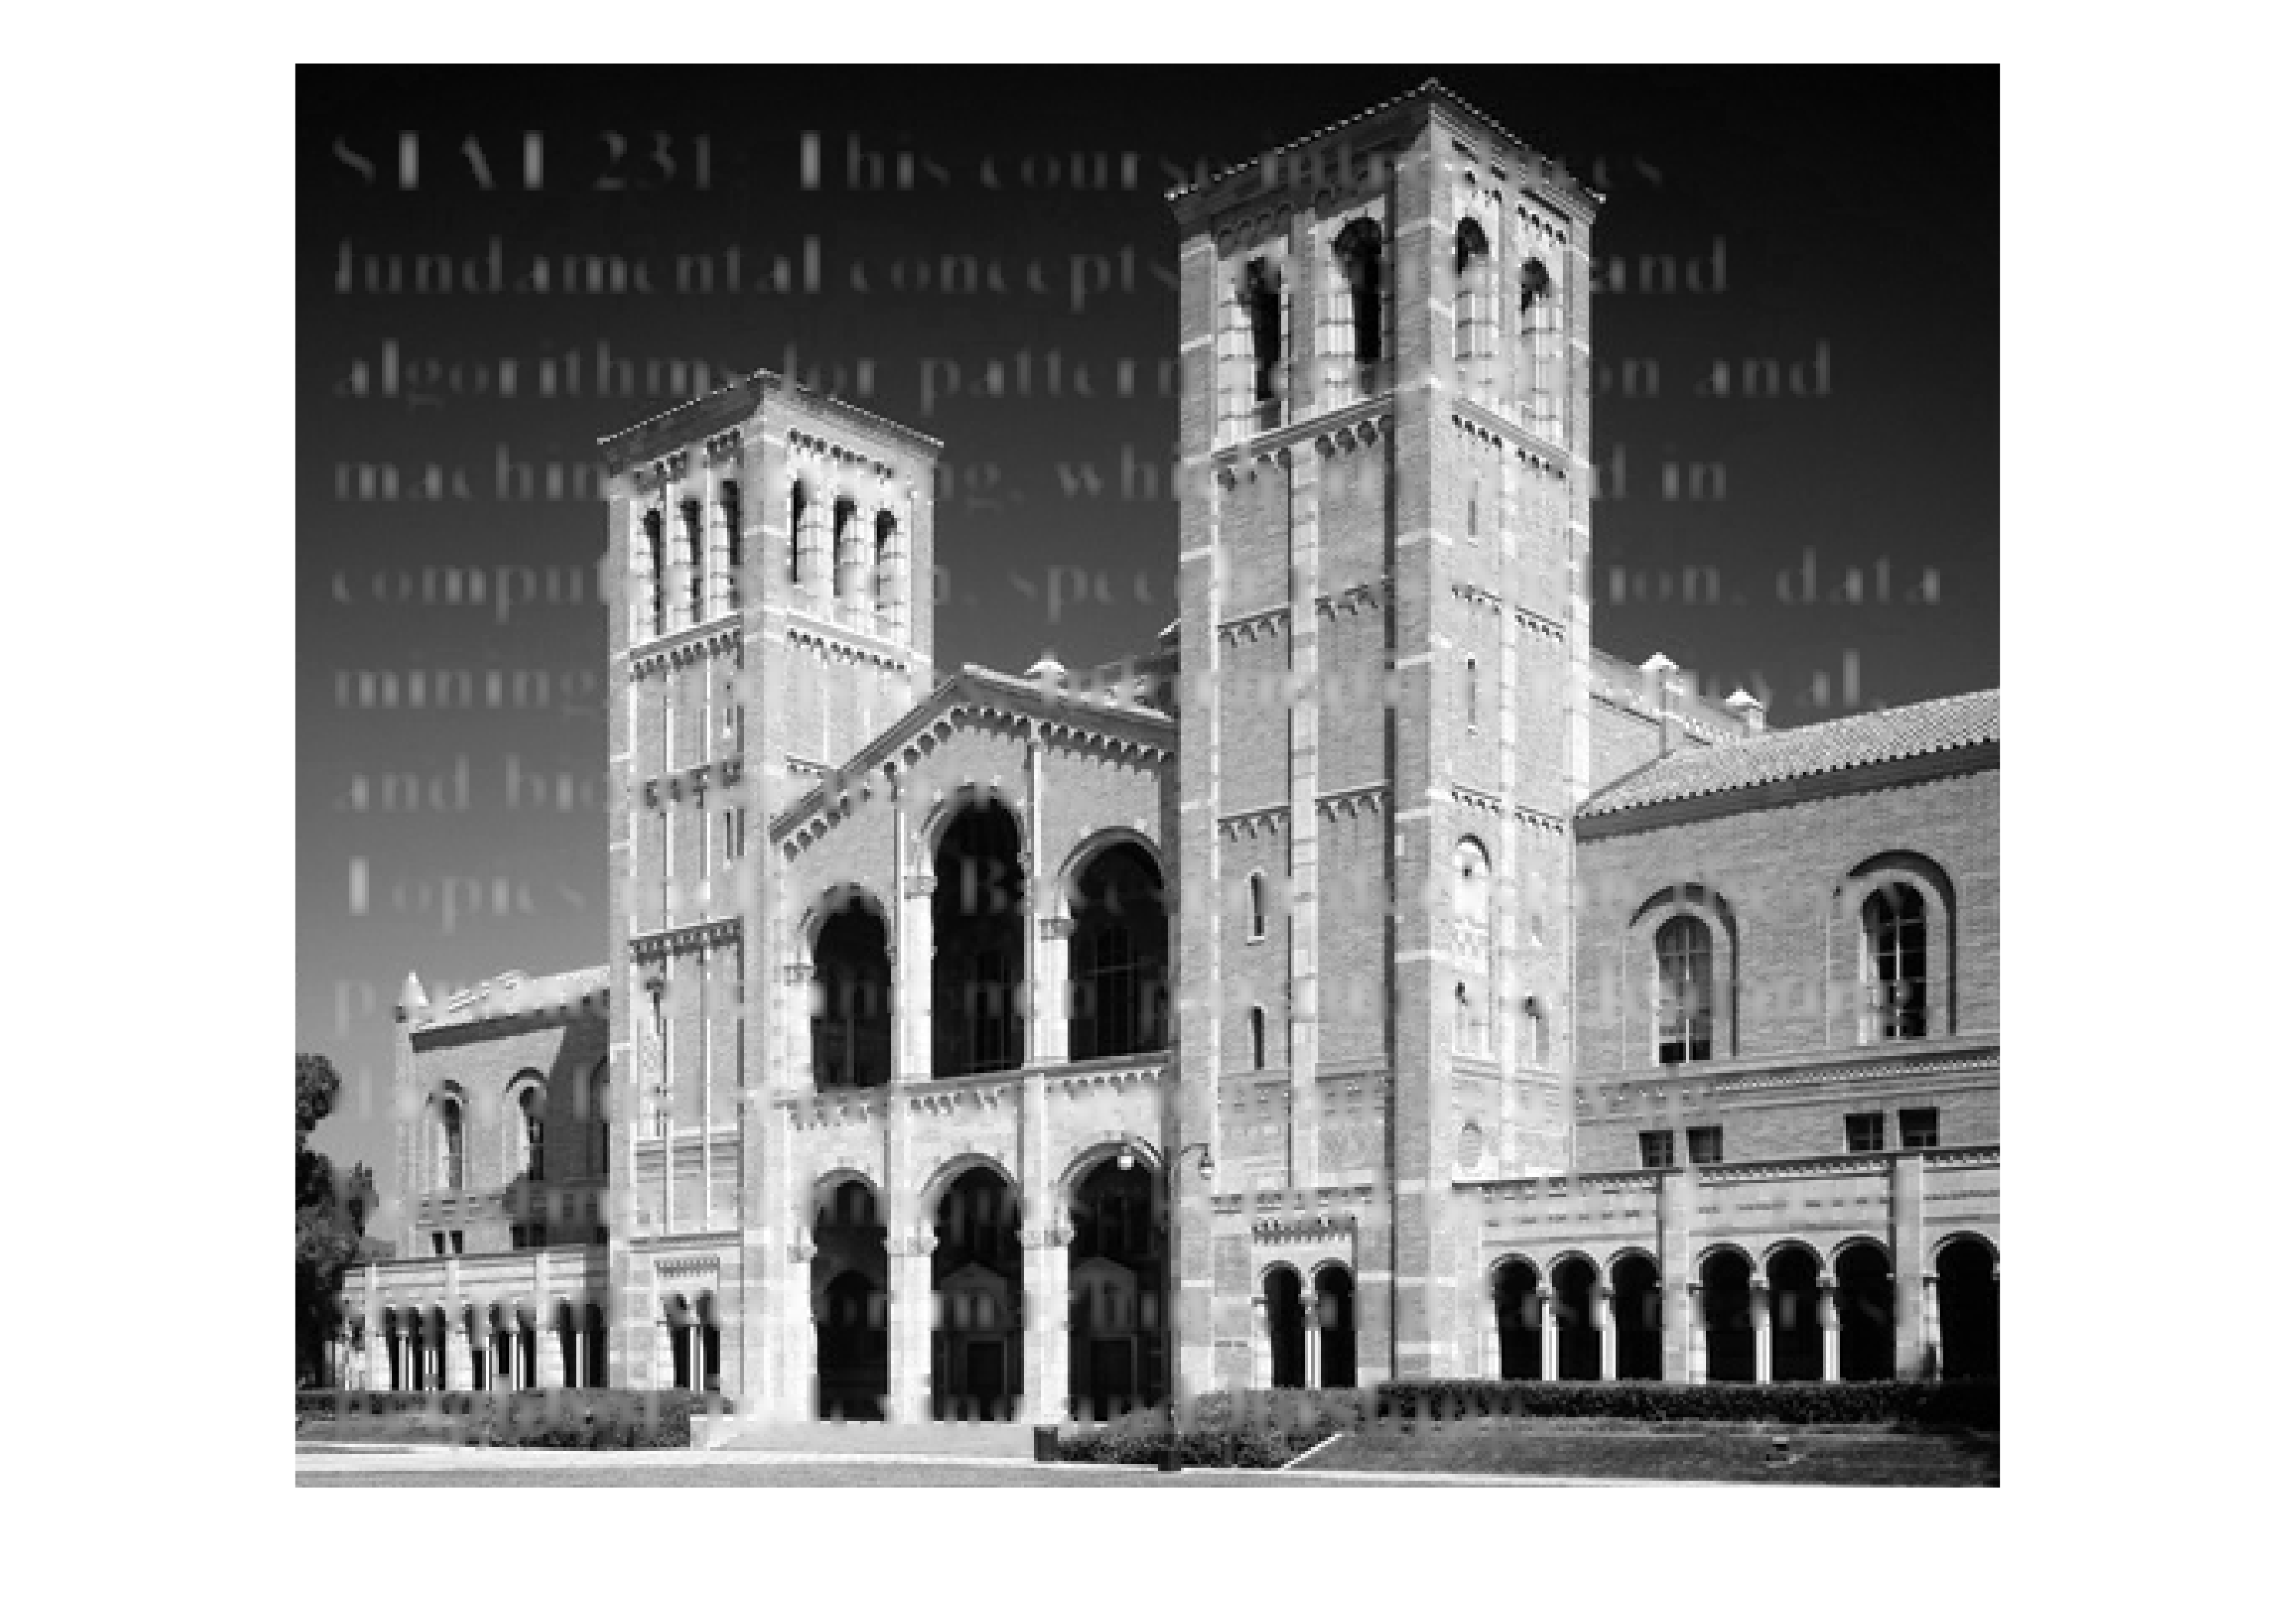
\includegraphics[width=\textwidth]{plot3_20}
        \caption{PDE Heat Equation 20 iterations}
        \label{fig:plot3_20}
    \end{subfigure}
    \begin{subfigure}[b]{0.49\textwidth}
        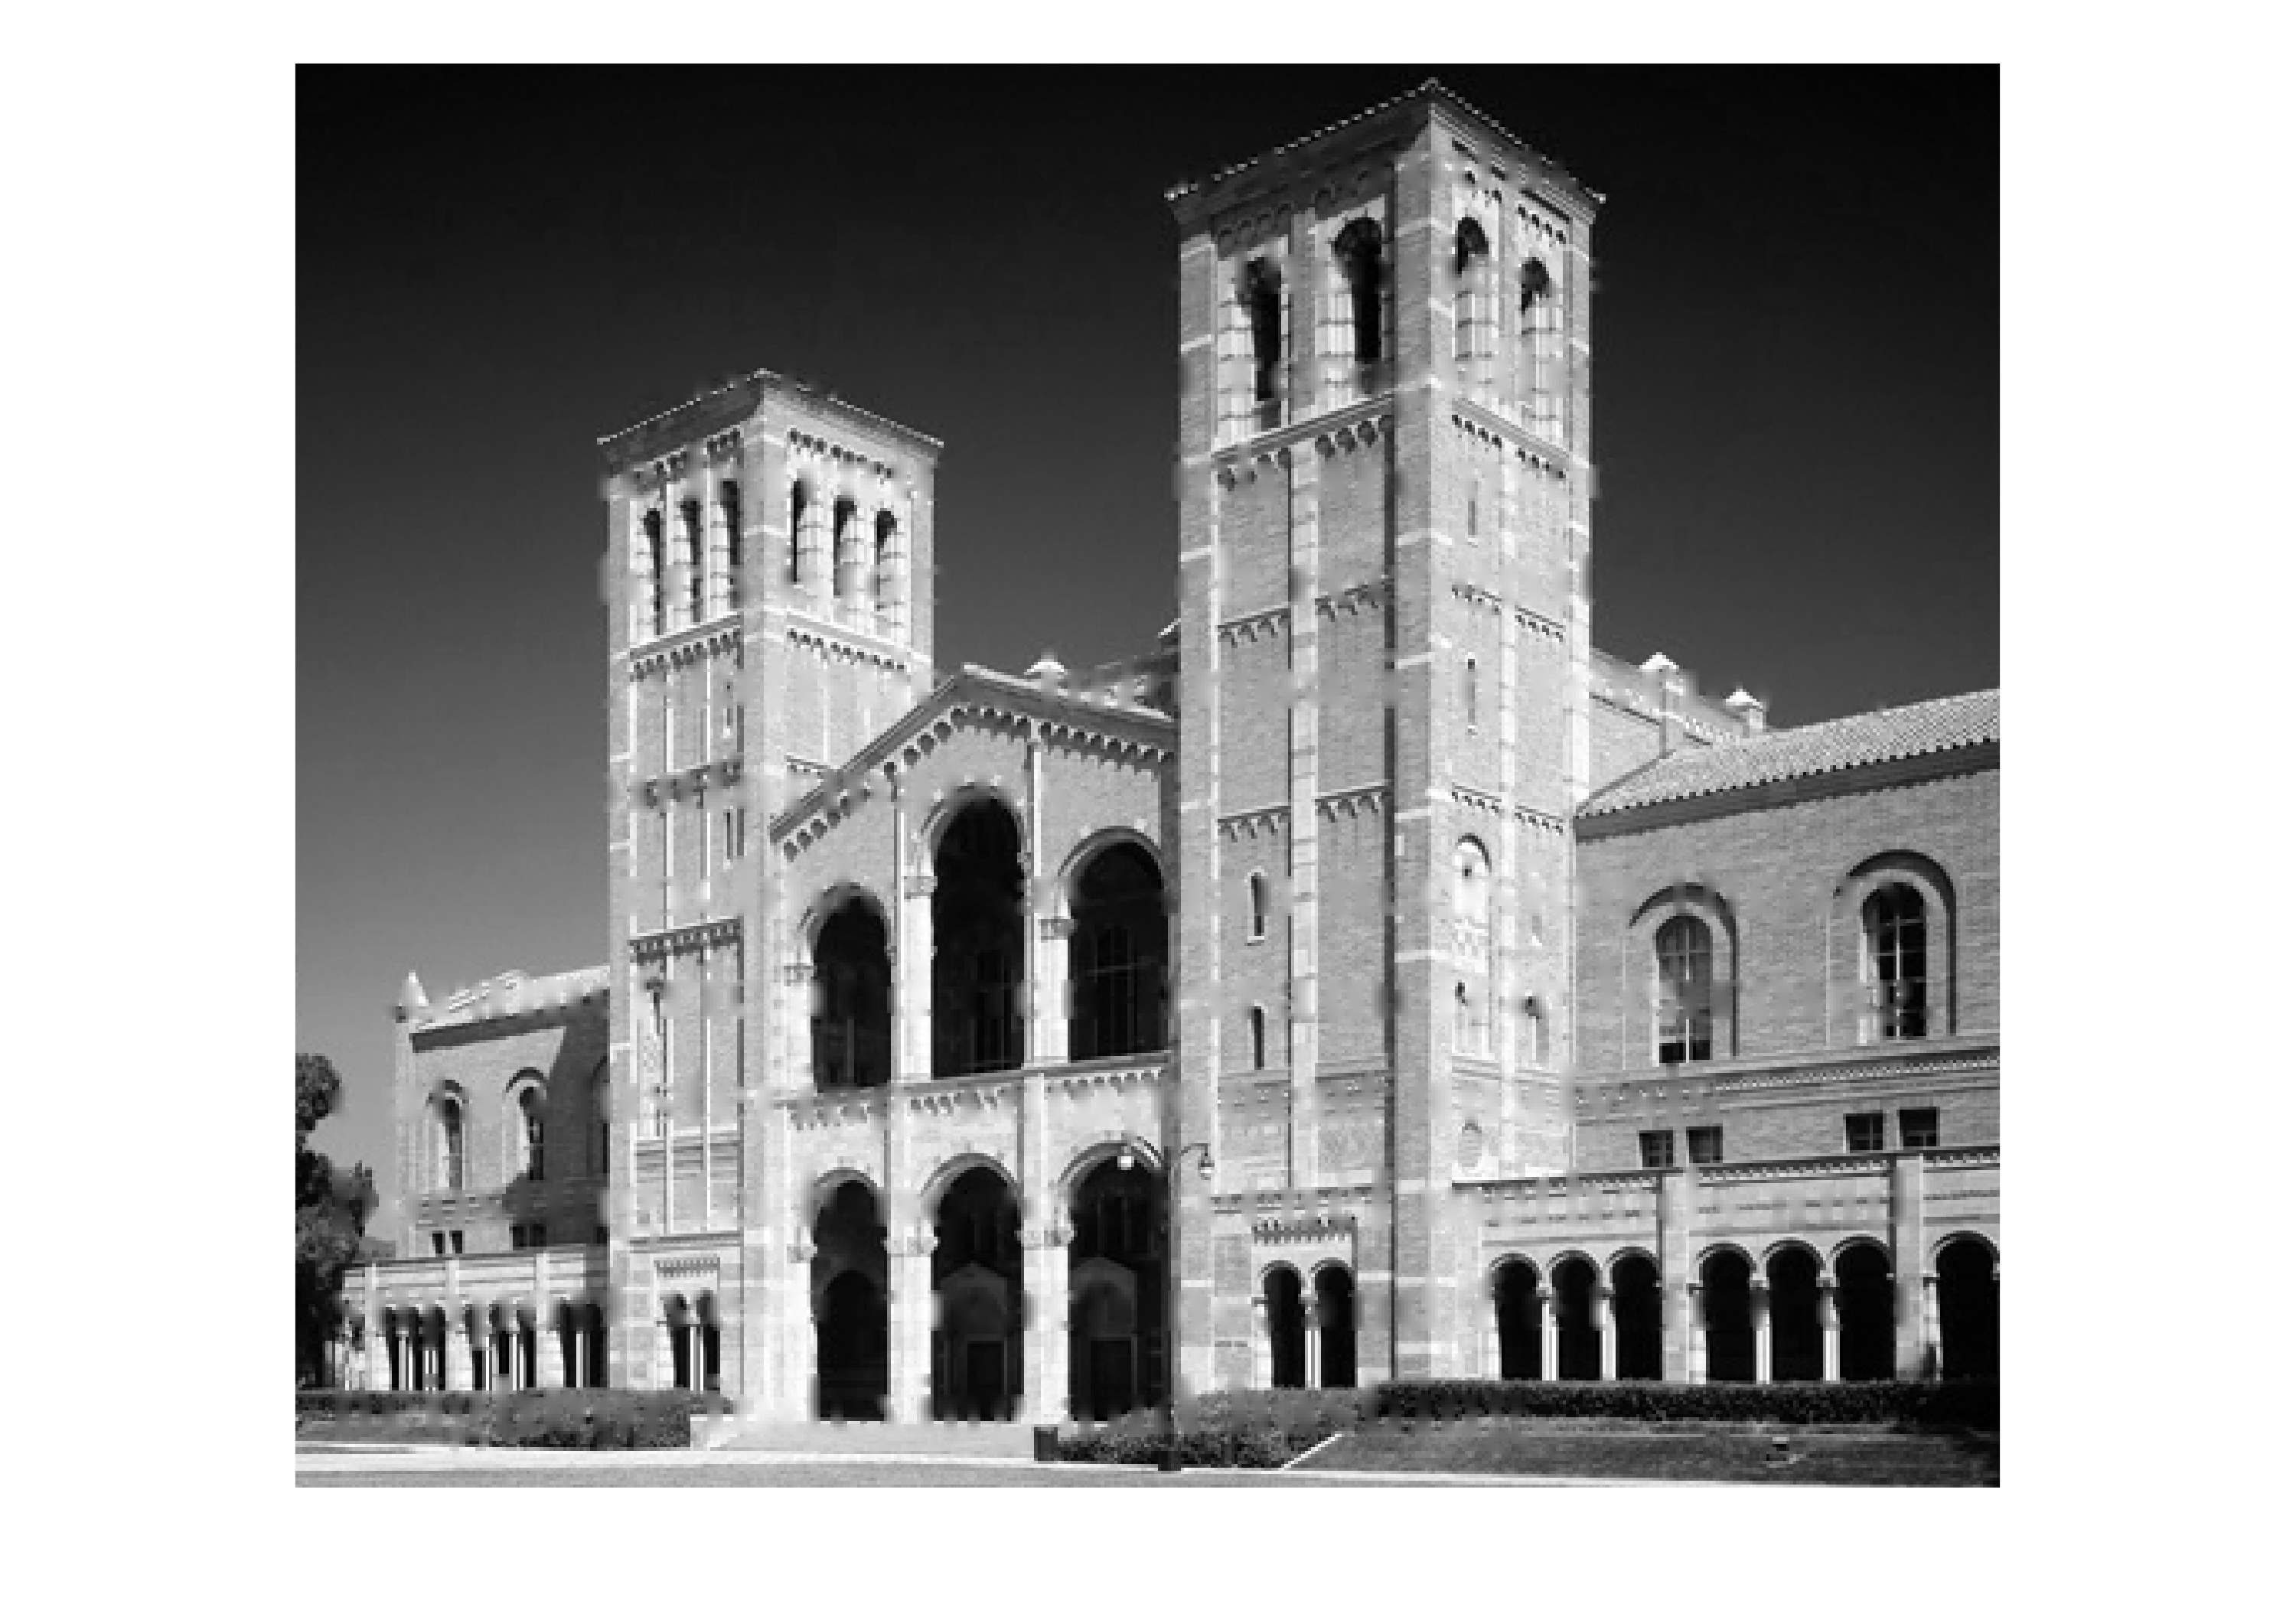
\includegraphics[width=\textwidth]{plot3_100}
        \caption{PDE Heat Equation 100 iterations}
        \label{fig:plot3_100}
    \end{subfigure}
    \caption{The restored results}\label{fig:results}
\end{figure}

\begin{figure}[H]
	\centering
	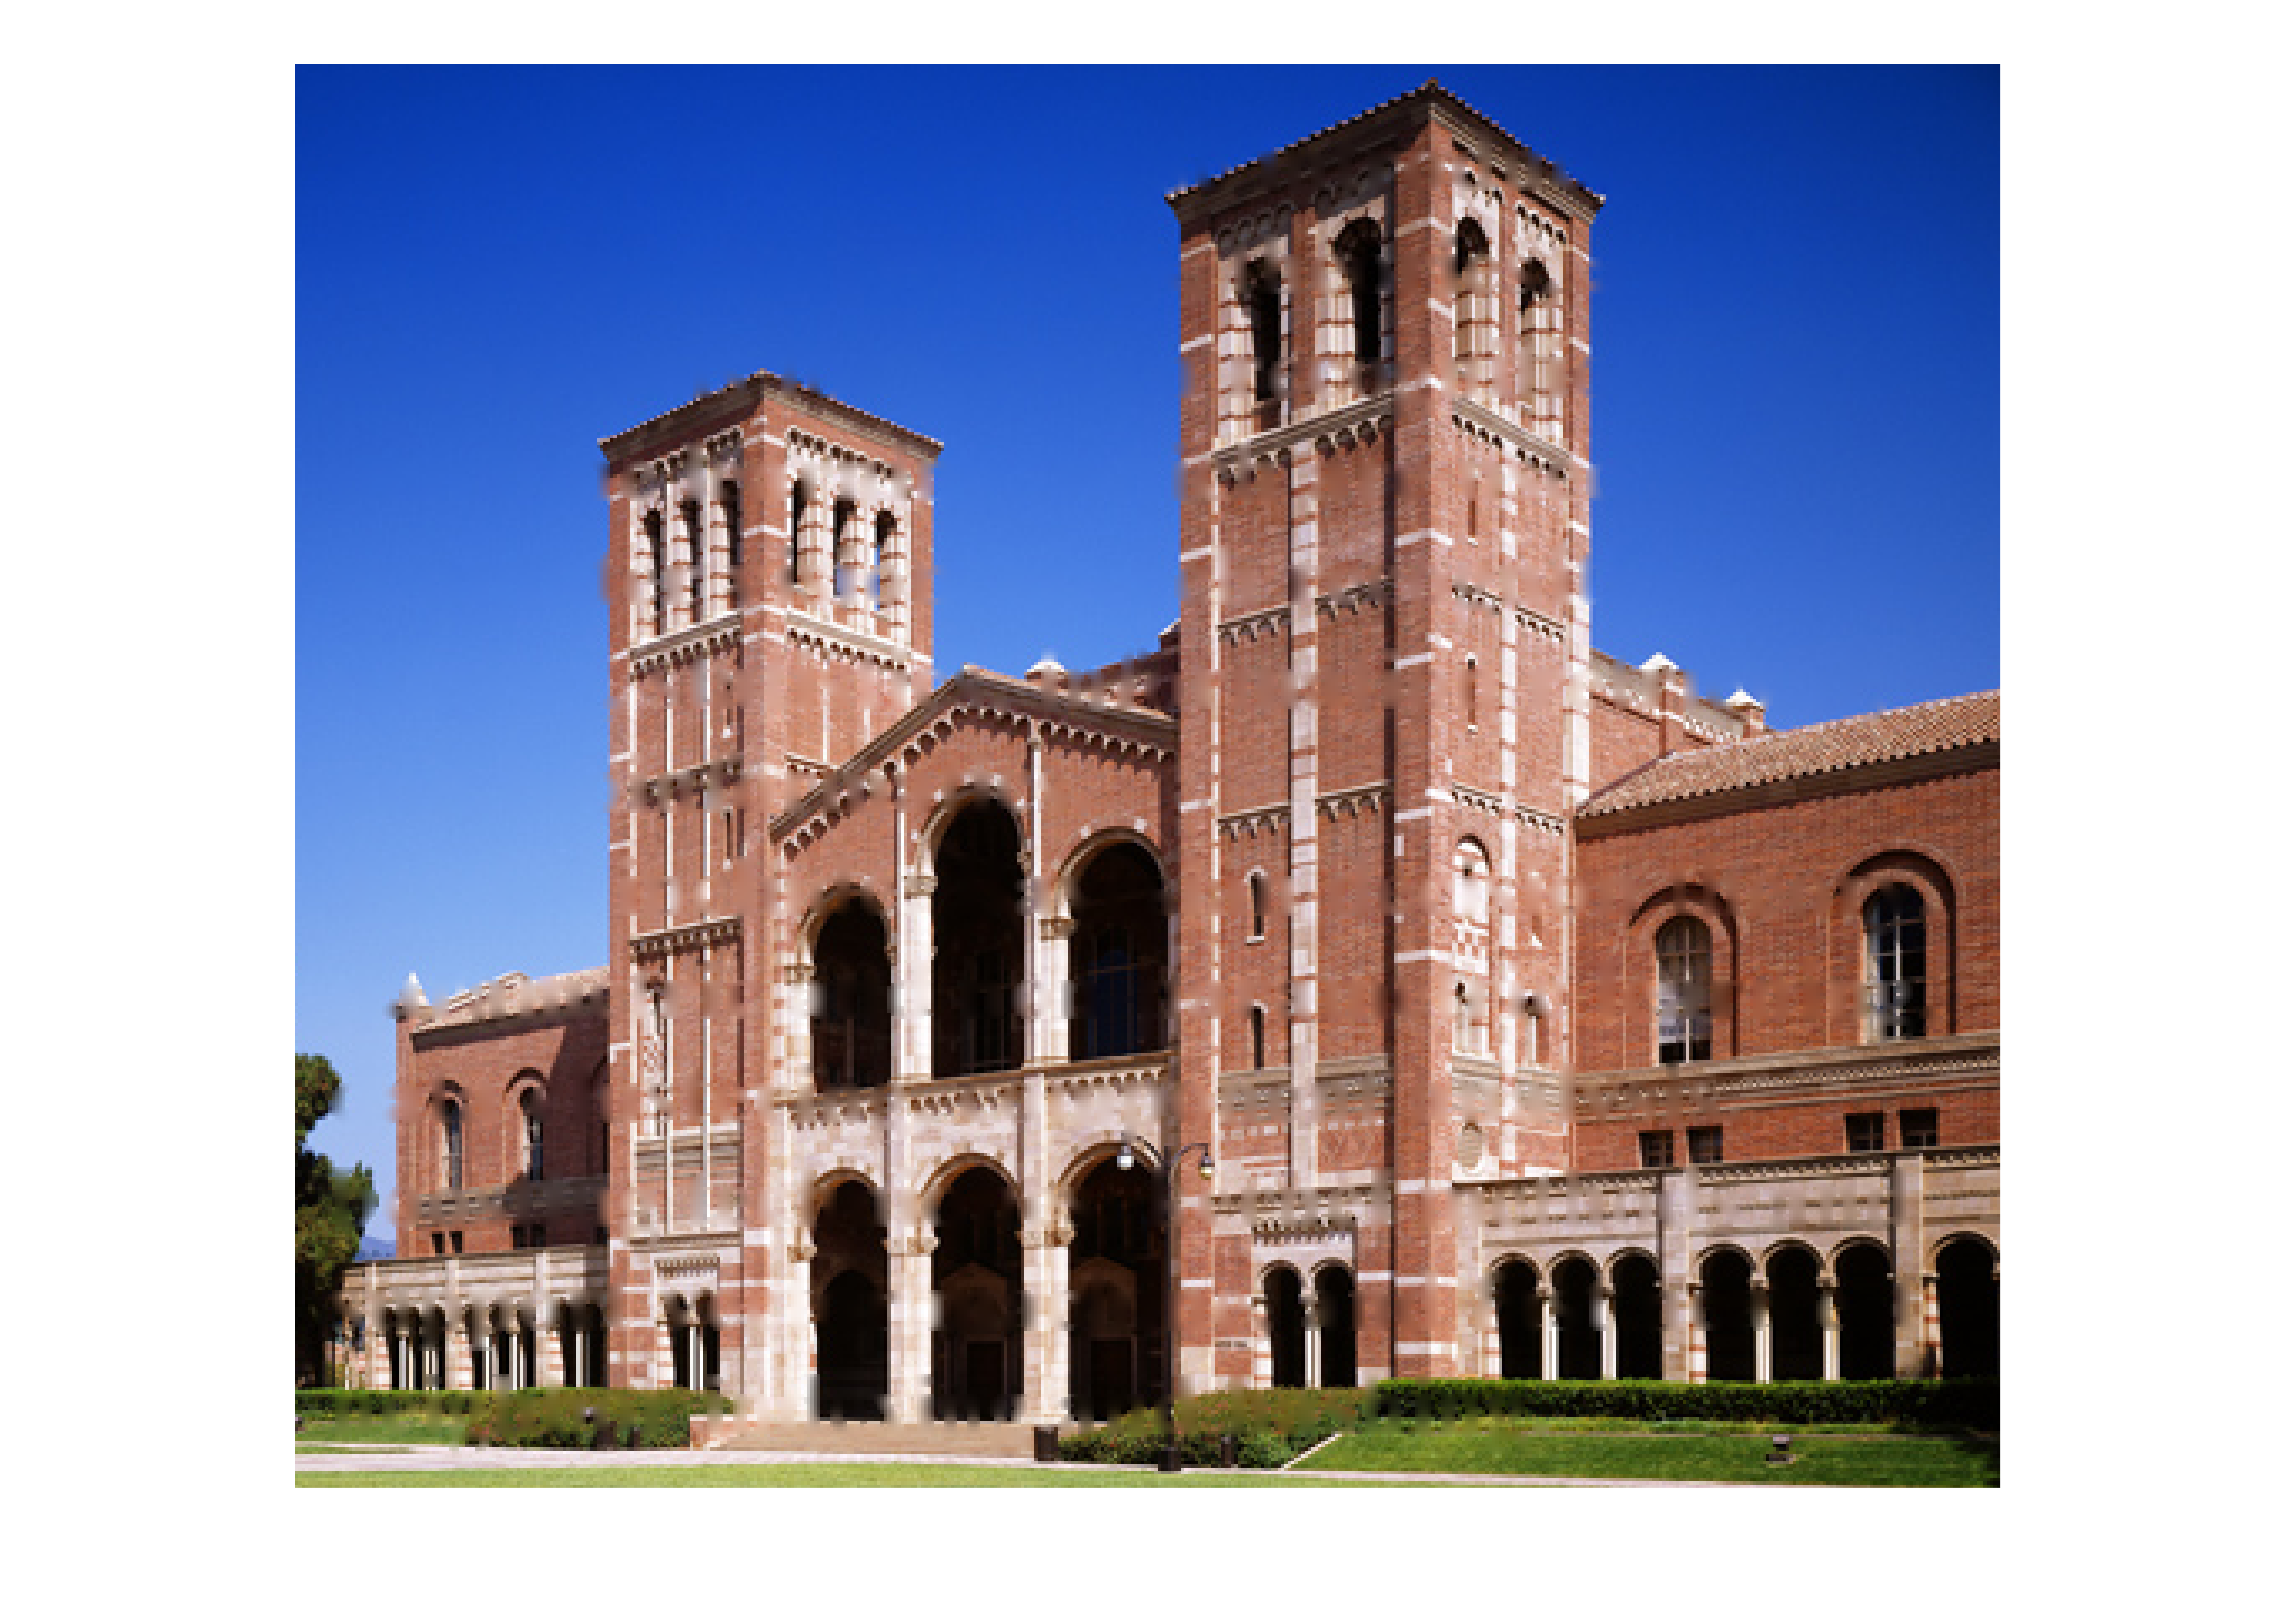
\includegraphics[width=0.9\textwidth]{plot4}
	\caption{The restored result of three channels}
	\label {fig:RGB}
\end{figure}
Figure \ref{fig:RGB} shows the restored result of three channels. As for colored images of RGB three channels, we need to sample from the joint distribution of the three random variables. However we notice that the potential energy of three channels (L1 or L2 norm) is the summation of the potential energies of one channel (componentwise L1 or L2 norm), which means the joint distribution is the product of the three marginal distributions. Thus, these three random variables are independent and then can be optimized separately. 
\end{document}  